\section{Auswertung}
\subsection{Wellenlängenbestimmung}
Die zur Bestimmung der Wellenlänge $\lambda$ aufgenommenen Werte sowie die daraus berechneten Wellenlängen sind in Tabelle \ref{welltab} dargestellt. Für $\lambda$ gilt hierbei
\begin{equation}
  \lambda = \frac{b}{n}\cdot\sin\left(\tan^{-1}\left(\frac{s_n}{L}\right)\right) \, .
\end{equation}
Hierbei bezeichnet n die Ordnung des Maximums, $b=\frac{1}{80}\,\si{\milli\meter}$ die Gitterbreite, $s_n$ den Abstand des $n$-ten Maximums zum $0$-ten Maximum und $L$ den Abstand zwischen Gitter und Schirm,
welcher hier $L=125\,\si{\centi\meter}$ beträgt.
\begin{table}[H]
  \centering
\begin{tabular}{c|c|c}
$n$  & $s_n$ [cm]    & $\lambda$ [nm]     \\
\hline
1 & 6,4 & 639,2 \\
2 & 6,3 & 631,7 \\
3 & 6,5 & 632,6 \\
4 & 6,5 & 629,3 \\
5 & 6,4 & 621,8 \\
6 & 6,5 & 614,7
\end{tabular}
\caption{Messwerte sowie berechnete Werte der Wellenlängenbestimmung.}
\label{welltab}
\end{table}
Als Mittelwert ergibt sich hierbei
\begin{equation}
  \lambda= (628,2 \pm 8,7) \, \si{\nano\meter}.
\end{equation}
\subsection{Modenuntersuchung}
\subsubsection{Grundmode}
Zur Untersuchung der Grundmode werden die Messwerte an eine Gaußfunktion der Form
\begin{equation}
\label{eqn:gauß}
  I_{(0, 0)}(L) = I_0\exp\left(-2\left(\frac{L - d_0}{\omega}\right)^2\right)
\end{equation}
gefittet. Hierbei bezeichnet $I_0$ die Maximalintensität, $d_0$ die Verschiebung der Photodiode senkrecht zur Strahlebene und $\omega$ den Strahlradius.\\
Mit den Messwerten aus Tabelle aus der folgenden Tabelle ergibt sich:
\begin{align*}
  I &=(1,04 \pm 0,04)\, \si{\micro\ampere}\\
  d &=(6,8 \pm 0,2)\, \si{\milli\meter}   \\
 \omega &=(6,6 \pm 0,3)\,  \si{\micro\ampere}
\end{align*}
\begin{table}
\begin{tabular}{c|c}
L [$ \si{\milli\meter}$]   &   I [$ \si{\micro\ampere}$]     \\
\hline
0  & 0,1444 \\
1  & 0,18   \\
2  & 0,37   \\
3  & 0,59   \\
4  & 0,765  \\
5  & 0,9    \\
6  & 0,85   \\
7  & 1,127  \\
8  & 0,97   \\
9  & 0,906  \\
10 & 0,667  \\
11 & 0,415  \\
12 & 0,269  \\
13 & 0,17   \\
14 & 0,083  \\
15 & 0,05
\end{tabular}
\caption{Die aufgenommenen Messwerte zur Untersuchung der Grundmode.}
\label{mode1}
\end{table}
Die Messwerte sowie der dazugehörige Fit sind in Abbildung $\ref{mode1fit}$ dargestellt.
\begin{figure}[H]
  \centering
  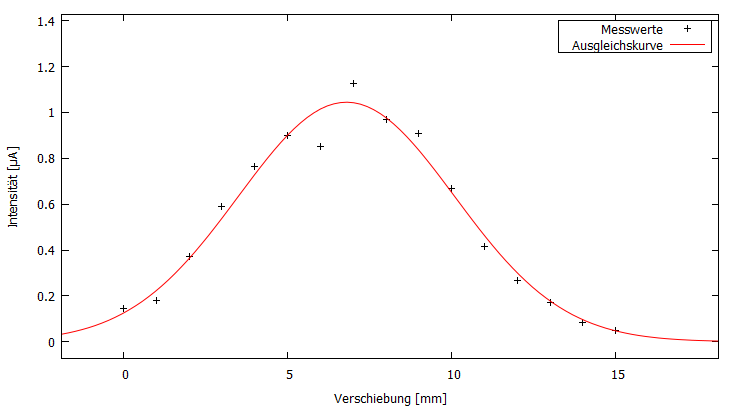
\includegraphics[width=14cm]{bilder/Grundmode.png}
  \caption{Messwerte sowie Fit zur Grundmode.}
  \label{mode1fit}
\end{figure}

\subsubsection{$\text{TEM}_{01}$-Mode}
Zur Untersuchung der $\text{TEM}_{01}$-Mode werden die aufgenommenen Messwerte aus Tabelle \ref{mode2} mit einer Funktion der Form
\begin{equation}
  I(L)=I_{0,1}\cdot\symup{e}^{\frac{-2(l-d_{0,1})^2}{(\omega_1)^2}}+I_{0,2}\cdot\symup{e}^{\frac{-2(l-d_{0,2})^2}{(\omega_2)^2}} \, ,
\end{equation}
wobei die Bedeutungen von $I_{0,1}$, $I_{0,2}$, $d_{0,1}$ $d_{0,2}$ und $\omega_1$ sowie $\omega_2$ analog zu denen bei der Grundmode sind, gefittet.
Es ergibt sich hierbei
\begin{align*}
 I_{0,1} &=(0,34 \pm 0,04)\, \si{\micro\ampere}\\
 d_{0,1} &=(4,29 \pm 0,22)\, \si{\milli\meter}\\
\omega_1 &=(3,2 \pm 0,4)\,  \si{\micro\ampere}\\
I_{0,2} &=(0,41 \pm 0,04)\, \si{\micro\ampere}\\
d_{0,2} &=(12,94 \pm 0,21)\, \si{\milli\meter}\\
\omega_2 &=(3,4 \pm 0,5)\,  \si{\micro\ampere}.
\end{align*}

\begin{table}[]
  \centering
\begin{tabular}{c|c}
L [$ \si{\milli\meter}$]   &   I [$ \si{\micro\ampere}$]     \\
  \hline
0  & 0,088  \\
1  & 0,135  \\
2  & 0,112  \\
3  & 0,17   \\
4  & 0,4    \\
5  & 0,3    \\
6  & 0,202  \\
7  & 0,07   \\
8  & 0,0093 \\
9  & 0,0178 \\
10 & 0,091  \\
11 & 0,218  \\
12 & 0,38   \\
13 & 0,41   \\
14 & 0,29   \\
15 & 0,25
\end{tabular}
\caption{Messwerte zur Untersuchung der ersten angeregten Mode.}
\label{mode2}
\end{table}
Die Ausgleichskurve ist zusammen mit den Messwerten in Abbildung \ref{mode2fit} dargestellt.
\begin{figure}[H]
  \centering
  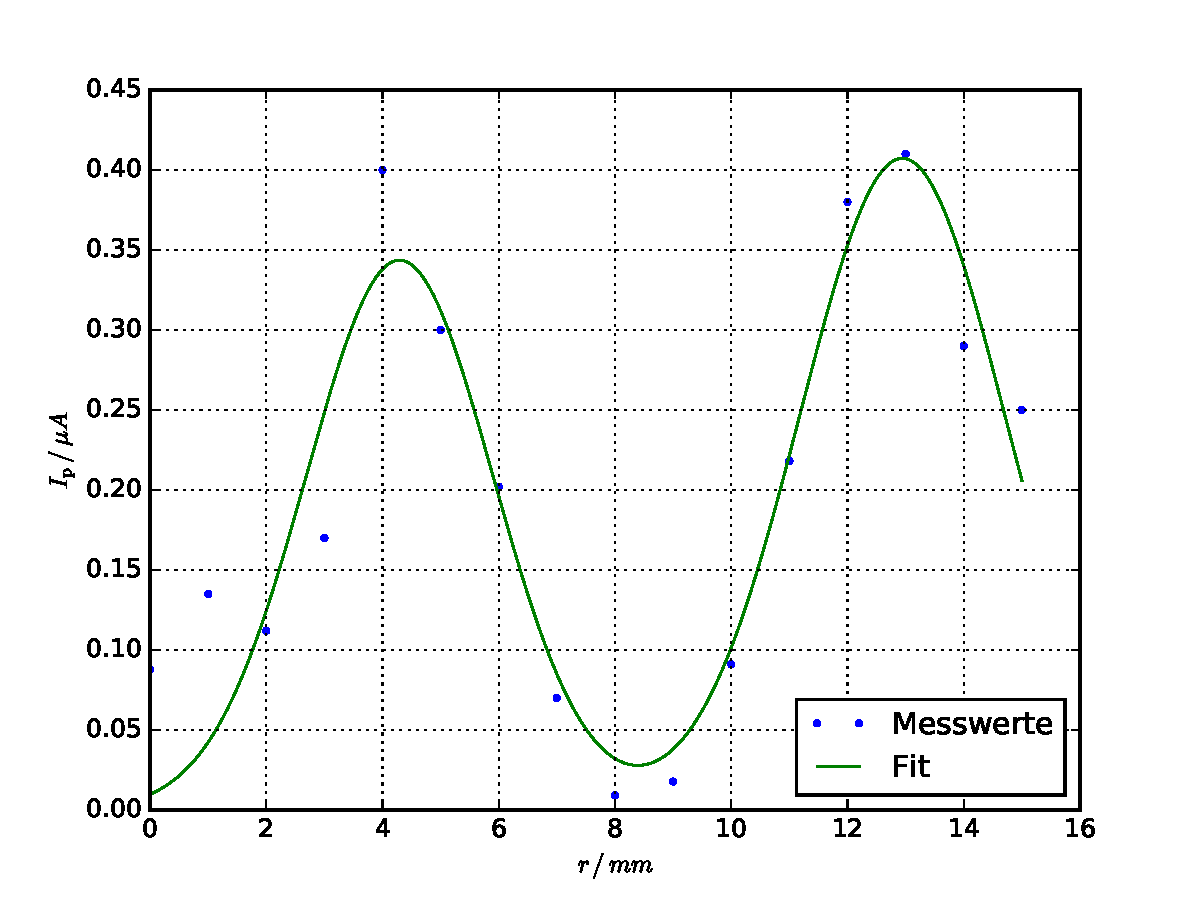
\includegraphics[width=14cm]{bilder/T_10.pdf}
  \caption{Messwerte und Fit der  $\text{TEM}_{01}$-Mode.}
  \label{mode2fit}
\end{figure}
\subsection{Polarisationsmessung}
Zur Untersuchung der Polarisation des Lasers werden die aufgenommenen Messwerte an eine Funktion der Form
\begin{equation}
   I(\varphi) = I_0 \cos^2\!\left(\varphi-\varphi_0\right)\,
\end{equation}
gefittet. Die in Abbiödung \ref{polfit} dargestellte Ausgleichsrechnung ergibt
\begin{align*}
 I_0 &=(2,68 \pm 0,05)\, \si{\micro\ampere}\\
 \varphi_0 &=72.5° \pm 0,96°.
\end{align*}
\begin{figure}[H]
  \centering
  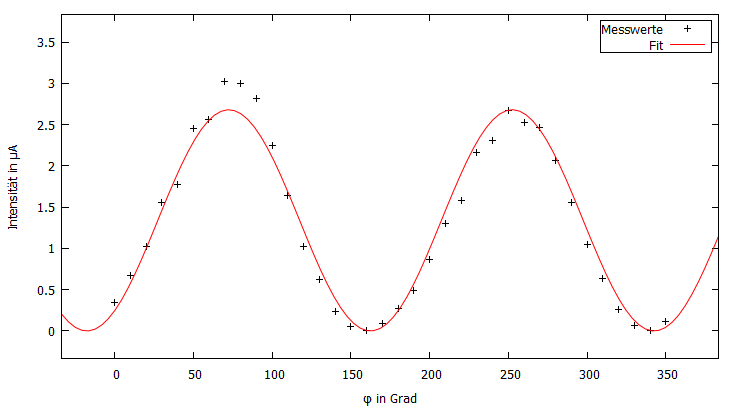
\includegraphics[width=14cm]{bilder/polarplot.png}
  \caption{Messwerte und Fit für die Polarisationsuntersuchung.}
  \label{polfit}
\end{figure}
Die aufgenommenen Messwerte finden sich in Tabelle \ref{polwert}.
\begin{table}[H]
  \centering
\begin{tabular}{c|c}
  Winkel [°]  &  Intensität [$ \si{\micro\ampere}$]     \\
  \hline
0   & 0,35  \\
10  & 0,67  \\
20  & 1,024 \\
30  & 1,555 \\
40  & 1,78  \\
50  & 2,45  \\
60  & 2,56  \\
70  & 3,02  \\
80  & 2,999 \\
90  & 2,815 \\
100 & 2,25  \\
110 & 1,637 \\
120 & 1,021 \\
130 & 0,619 \\
140 & 0,231 \\
150 & 0,058 \\
160 & 0,005 \\
170 & 0,096 \\
180 & 0,27  \\
190 & 0,492 \\
200 & 0,864 \\
210 & 1,306 \\
220 & 1,582 \\
230 & 2,156 \\
240 & 2,31  \\
250 & 2,667 \\
260 & 2,527 \\
270 & 2,46  \\
280 & 2,069 \\
290 & 1,557 \\
300 & 1,052 \\
310 & 0,636 \\
320 & 0,26  \\
330 & 0,063 \\
340 & 0,007 \\
350 & 0,11
\end{tabular}
\caption{Messwerte zur Untersuchung der Polarisation.}
\label{polwert}
\end{table}
\subsection{Stabilitätsmessung}
Bei der ersten untersuchten Spiegelkonfiguration handelt es sich um zwei konkave Spiegel. Die aufgenommenen Messwerte werden an eine Funktion der Form
\begin{equation}
  I(s)=a\cdot s^2+bs+c
\end{equation}
gefittet. Dies ist in Abbildung \ref{stabfit1} dargestellt. Die Ausgleichsrechnung ergibt
\begin{align*}
 a &=(0,0017 \pm 0,0007)\, \frac{\si{\micro\ampere}}{\si{\centi\meter}^2}\\
 b &=(-0,4 \pm 0,2)\,  \frac{\si{\micro\ampere}}{\si{\centi\meter}}\\
  c &=(22,1+- 7,1)\,  \si{\micro\ampere}.
\end{align*}
\begin{figure}[H]
  \centering
  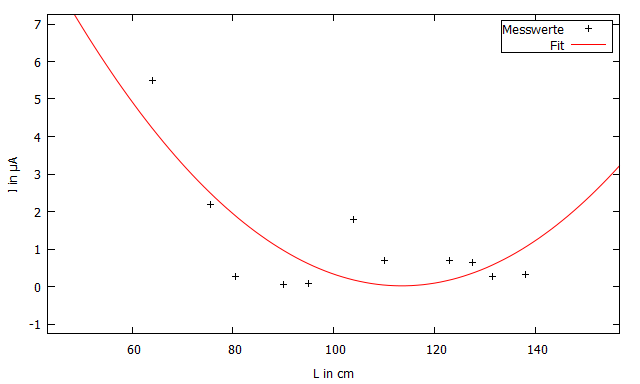
\includegraphics[width=14cm]{bilder/konkavkonkav.png}
  \caption{Messwerte und Fit für die Stabilitätsmessung mit zwei konkaven Spiegeln.}
  \label{stabfit1}
\end{figure}
Die zweite Spiegelkonfiguration besteht aus einem konkaven und einem planaren Spiegel. Hierbei wird als Fitfunktion eine lineare Funktion der Form
\begin{equation}
  I(s)=m\cdot s+b
\end{equation}
verwandt. Es ergibt sich:
\begin{align*}
  m &=(-0,004 \pm 0,02)\,  \frac{\si{\micro\ampere}}{\si{\centi\meter}}\\
  b &=(0,91 \pm 1,4)\,\si{\micro\ampere}.\\
\end{align*}
Die Messwerte mit Ausgleichsgerade sind in Abbildung \ref{dumm} dargestellt.
\begin{figure}[H]
  \centering
  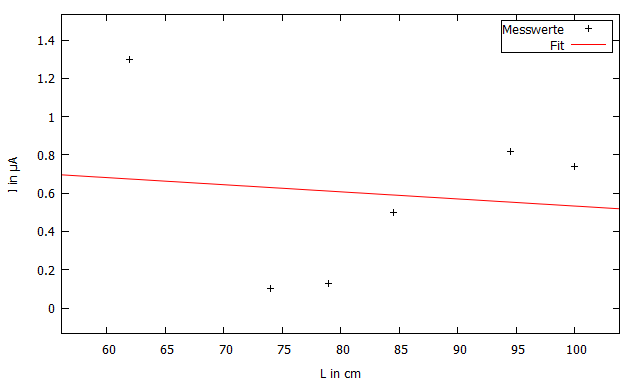
\includegraphics[width=14cm]{bilder/konkavplanar.png}
  \caption{Messwerte und Fit für die Stabilitätsmessung mit einem konkaven und einem konvexen Spiegel.}
  \label{dumm}
\end{figure}
